\documentclass{article}
\usepackage[utf8]{inputenc}
\usepackage{fancyvrb}
\usepackage{url}
\usepackage{graphicx}
\usepackage{grffile}
\usepackage{float}
\usepackage{natbib}
%% \VignetteIndexEntry{Roxygen Vignette}
\newcommand{\Roxygen}{\texttt{Roxygen}}
%% path, filename, caption, label
\newcommand{\listing}[4]{        %
  \begin{figure}[H]              %
    \centering                   %
    \VerbatimInput[numbers=left, %
      frame=single,              %
      label=#2]{#1}              %
    \caption{#3}                 %
    \label{#4}                   %
  \end{figure}                   %
}
\author{Peter Danenberg \url{<pcd@roxygen.org>}}
\title{\Roxygen{} Vignette}
\usepackage{Sweave}
\begin{document}
\maketitle
\begin{abstract}
  The purpose of the \Roxygen{} Vignette is to show how to get up and
  running with \Roxygen{}; for details, including a complete list of
  tags, consult the help pages or manual for:
  \begin{itemize}
  \item \texttt{make.callgraph.roclet}
  \item \texttt{make.collate.roclet}
  \item \texttt{make.namespace.roclet}
  \item \texttt{make.Rd.roclet}
  \end{itemize}
\end{abstract}
\tableofcontents
\section{Minimal Example: ``Hello, Roxygen!''}

\listing{hello-roxygen.R}
        {hello-roxygen.R}
        {Roxygen sanity-check}
        {hello-roxygen}

\texttt{hello-roxygen.R} (fig. \ref{hello-roxygen}) is a minimal
example to check the sanity of your \Roxygen{} installation. It merely
replaces the package description so that `\texttt{R CMD check}' will
run after \Roxygen{} has processed the package skeleton:

\begin{Schunk}
\begin{Sinput}
> library(roxygen)
> package.skeleton('helloRoxygen',
+                  code_files='hello-roxygen.R',
+                  force=TRUE)
> # `R CMD roxygen -d helloRoxygen' works, too.
> roxygenize('helloRoxygen',
+            roxygen.dir='helloRoxygen',
+            copy.package=FALSE,
+            unlink.target=FALSE)
\end{Sinput}
\begin{Soutput}
Writing helloRoxygen-package to helloRoxygen/man/helloRoxygen-package.Rd
Writing namespace directives to helloRoxygen/NAMESPACE 
Merging collate directive with helloRoxygen/DESCRIPTION to helloRoxygen/DESCRIPTION 
\end{Soutput}
\end{Schunk}

A new \texttt{helloRoxygen/man/helloRoxygen-package.Rd} should have
been created with the contents of figure \ref{hello-roxygen}; and
`\texttt{R CMD check helloRoxygen}' should terminate successfully.

\section{Example: Pseudoprimality}

\subsection{Package Description}

\listing{pseudoprime/R/pseudoprime-package.R}
        {pseudoprime-package.R}
        {Package description for \texttt{pseudoprime}}
        {pseudoprime-package}

One could imagine, for instance, a less trivial package that actually
does something; enter \texttt{pseudoprime}, a toy that tests for
primes using Fermat's little
theorem.\footnote{\url{http://en.wikipedia.org/wiki/Fermat's_little_theorem}}

A package description has been provided in figure
\ref{pseudoprime-package}; notice the \texttt{roxygen()} statement in
line 30: each \Roxygen{} description block must be followed by a
statement, even header material that describes a file or package in
lieu of a specific function. \texttt{roxygen()} is provided as a
\texttt{NOOP} (null statement) to stand in for such cases.

The first sentence of any \Roxygen{} block briefly describes its
object; and may be followed directly by a \Roxygen{} tag
(fig. \ref{hello-roxygen}, line 2) or a more detailed description
(fig.  \ref{pseudoprime-package}, line 3). The detailed description
begins after the intervening blank line, and continues until the first
\Roxygen{} tag (fig. \ref{pseudoprime-package}, line 19).

Each \Roxygen{} tag begins with an asperand, like \texttt{@name},
\texttt{@author}, etc.; which means, incidentally, that all real
asperands have to be escaped with a double-asperand, as in
\verb=\email{pcd@@roxygen.org}= (fig. \ref{pseudoprime-package}, line
23).

Furthermore, although \Roxygen{} tags replace many of the structural
Rd elements such as \verb=\title=, \verb=\keyword=, etc.; stylistic Rd
elements such as \verb=\emph= and \verb=\email= can be used freely
within \Roxygen{} tags. See ``Writing R Extensions'' for
details. \citep[\S2.3 ``Marking text'']{r-core}

\subsection{Fermat Test}

\listing{pseudoprime/R/fermat.R}
        {fermat.R}
        {Roxygen example \texttt{fermat.R}}
        {fermat}


When documenting functions (fig. \ref{fermat}), every parameter must
be documented with a \texttt{@param} tag (line 8); which consists of
\texttt{@param <variable> <description>}. Similarly, the return value
must be documented with \texttt{@return <description>} (lines 9-10).

Notice \texttt{@callGraphPrimitives} (line 11): it creates a call
graph at the default depth similar to figure \ref{fermat-test},
including primitive functions; \texttt{@callGraph}, on the other hand,
would exclude primitive functions. Note that this roclet requires
package {\tt Rgraphviz} $\geq 1.19.2$, and with {\tt Roxygen} $0.1-1$
the {\tt callgraph} roclet is not automatically executed anymore; see
help for function {\tt make.callgraph.roclet}\ref{running}.

%\begin{figure}[H]
%  \centering
%  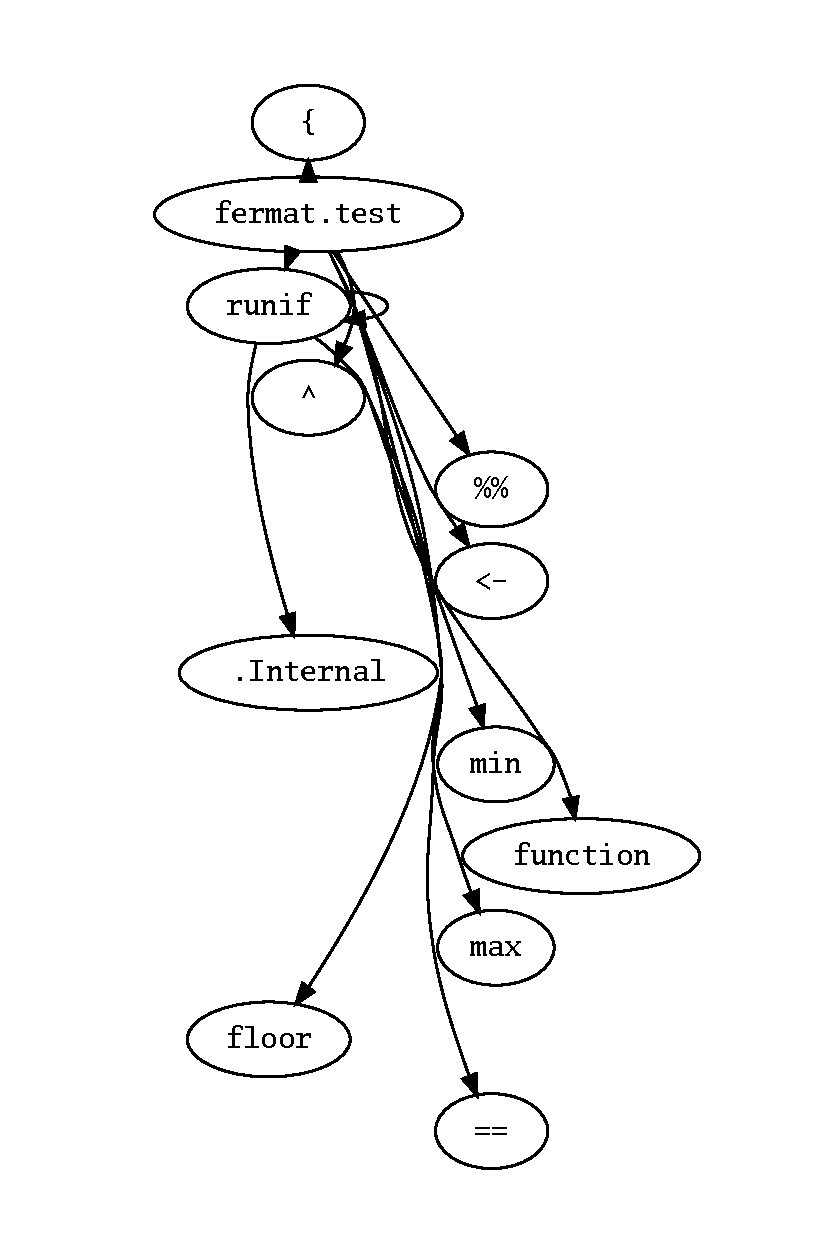
\includegraphics{pseudoprime/inst/doc/fermat.test-callgraph.pdf}
%  \caption{\texttt{fermat.test} call graph with primitives}
%  \label{fermat-test}
%\end{figure}

\subsection{Pseudoprime}

\listing{pseudoprime/R/pseudoprime.R}
        {pseudoprime.R}
        {Roxygen example \texttt{pseudoprime.R}}
        {pseudoprime}

Notice the header in \texttt{pseudoprime.R} (fig. \ref{pseudoprime})
terminated by \texttt{roxygen()}; \texttt{@include fermat.R} (line 1)
signals that \texttt{fermat.R} should be loaded before
\texttt{pseudoprime.R}.  The collate roclet will update
\texttt{DESCRIPTION} accordingly.

\texttt{@export} (line 15) signifies that \texttt{is.pseudoprime} will
be added to an export directive in \texttt{NAMESPACE}.

\subsection{Running \Roxygen{}}

Running \texttt{`R CMD roxygen -d pseudoprime'} populates \texttt{man}
with Rd files, edits \texttt{DESCRIPTION} and \texttt{NAMESPACE}, and
puts call graphs in \texttt{inst/doc}:

\begin{Schunk}
\begin{Soutput}
Writing fermat.test to pseudoprime/man/fermat.test.Rd
Writing pseudoprime-package to pseudoprime/man/pseudoprime-package.Rd
Writing is.pseudoprime to pseudoprime/man/is.pseudoprime.Rd
Writing namespace directives to pseudoprime/NAMESPACE 
Merging collate directive with pseudoprime/DESCRIPTION to pseudoprime/DESCRIPTION 
\end{Soutput}
\end{Schunk}

The \texttt{roxygenize} function is an alternative to \texttt{`R CMD
  roxygen'}; see the help page for details.


\bibliographystyle{plainnat}
\bibliography{roxygen}
\end{document}
